%\VignetteEngine{knitr::knitr}
%\VignetteIndexEntry{ESGtoolkit}
\documentclass[a4paper]{article}\usepackage[]{graphicx}\usepackage[]{color}
% maxwidth is the original width if it is less than linewidth
% otherwise use linewidth (to make sure the graphics do not exceed the margin)
\makeatletter
\def\maxwidth{ %
  \ifdim\Gin@nat@width>\linewidth
    \linewidth
  \else
    \Gin@nat@width
  \fi
}
\makeatother

\definecolor{fgcolor}{rgb}{0.345, 0.345, 0.345}
\newcommand{\hlnum}[1]{\textcolor[rgb]{0.686,0.059,0.569}{#1}}%
\newcommand{\hlstr}[1]{\textcolor[rgb]{0.192,0.494,0.8}{#1}}%
\newcommand{\hlcom}[1]{\textcolor[rgb]{0.678,0.584,0.686}{\textit{#1}}}%
\newcommand{\hlopt}[1]{\textcolor[rgb]{0,0,0}{#1}}%
\newcommand{\hlstd}[1]{\textcolor[rgb]{0.345,0.345,0.345}{#1}}%
\newcommand{\hlkwa}[1]{\textcolor[rgb]{0.161,0.373,0.58}{\textbf{#1}}}%
\newcommand{\hlkwb}[1]{\textcolor[rgb]{0.69,0.353,0.396}{#1}}%
\newcommand{\hlkwc}[1]{\textcolor[rgb]{0.333,0.667,0.333}{#1}}%
\newcommand{\hlkwd}[1]{\textcolor[rgb]{0.737,0.353,0.396}{\textbf{#1}}}%
\let\hlipl\hlkwb

\usepackage{framed}
\makeatletter
\newenvironment{kframe}{%
 \def\at@end@of@kframe{}%
 \ifinner\ifhmode%
  \def\at@end@of@kframe{\end{minipage}}%
  \begin{minipage}{\columnwidth}%
 \fi\fi%
 \def\FrameCommand##1{\hskip\@totalleftmargin \hskip-\fboxsep
 \colorbox{shadecolor}{##1}\hskip-\fboxsep
     % There is no \\@totalrightmargin, so:
     \hskip-\linewidth \hskip-\@totalleftmargin \hskip\columnwidth}%
 \MakeFramed {\advance\hsize-\width
   \@totalleftmargin\z@ \linewidth\hsize
   \@setminipage}}%
 {\par\unskip\endMakeFramed%
 \at@end@of@kframe}
\makeatother

\definecolor{shadecolor}{rgb}{.97, .97, .97}
\definecolor{messagecolor}{rgb}{0, 0, 0}
\definecolor{warningcolor}{rgb}{1, 0, 1}
\definecolor{errorcolor}{rgb}{1, 0, 0}
\newenvironment{knitrout}{}{} % an empty environment to be redefined in TeX

\usepackage{alltt}
\usepackage[british]{babel}
\usepackage[sc]{mathpazo} % Use the Palatino font
\usepackage[utf8]{inputenc}
\usepackage[T1]{fontenc}
\usepackage[colorlinks,linkcolor=red, citecolor=blue, urlcolor=red]{hyperref}
\usepackage{xcolor}
\usepackage{url}
\usepackage{float}
\usepackage{amssymb,amsfonts,amsmath}
\usepackage{graphicx}
\usepackage{latexsym}
\usepackage[authoryear]{natbib}
\usepackage{fancyhdr} % Headers and footers
\pagestyle{fancy} % All pages have headers and footers
\fancyhead{} % Blank out the default header
\fancyhead[C]{\code{ESGtoolkit}, tools for stochastic simulation $\bullet$ January 2020} % 
\date{}
\newcommand{\CC}{\ensuremath{\mathbb{C}} }
\newcommand{\NN}{\ensuremath{\mathbb{N}} }
\newcommand{\RR}{\ensuremath{\mathbb{R}} }
\newcommand{\QQ}{\ensuremath{\mathbb{Q}} }
\newcommand{\EE}{\ensuremath{\mathbb{E}} }
\newcommand{\PP}{\ensuremath{\mathbb{P}} }
\newcommand{\noi}{\noindent}
\newcommand{\II}{\mbox{\large 1\hskip -0,353em 1}}
\newcommand{\dps}{\displaystyle}
\newcommand{\ms}{\medskip}
\newcommand{\itb}{\ms\item[$\bullet$]}
\newcommand{\itm}{\ms\item}
\newcommand{\pkg}[1]{{\normalfont\fontseries{b}\selectfont #1}}
\newcommand{\proglang}[1]{\textsf{#1}}
\newcommand{\code}[1]{\mbox{\texttt{#1}}}
\newcommand{\MN}{\mathcal{N}}
\newcommand{\MM}{\mathcal{M}}
\newcommand{\FF}{\mathcal{F}}
\newcommand{\GG}{\mathcal{G}}
\newcommand{\HH}{\mathcal{H}}
\newcommand{\LL}{\mathcal{L}}
\newcommand{\AT}{\mathcal{A}}
\IfFileExists{upquote.sty}{\usepackage{upquote}}{}
\begin{document}

\title{\bf{\code{ESGtoolkit}, a tool for stochastic simulation (\code{v0.2.0})}} % Article title
\author{
Thierry Moudiki\\ % Your name
%\url{http://thierrymoudiki.wordpress.com}\\ % Your institution
\today{}
%\href{mailto:thierry.moudiki@gmail.com}{thierry.moudiki@gmail.com} % Your email address
}
\maketitle

\tableofcontents

\newpage

\section{Overview}

\subsection{Context}

This package was initially developped for insurance in 2014. \textbf{If you're not working in insurance, this package is still relevant for stochastic simulation} in Finance, Economics, or Physics. In that case, you can start directly with \ref{sec:simdiff}. Oh, except maybe this paragraph: \ref{para}. 

\medskip

An \textit{Economic Scenario Generator} (ESG) is a tool for projection of plausible future paths for an insurer's financial risk factors. It helps in pricing its insurance products, and assessing current and future solvency. Two types of ESGs are generally needed, for different purposes : a \textit{real-world} ESG, and a  a \textit{market consistent} ESG.


\medskip

The aim of a real-world ESG is to produce projections of risk factors, whose distribution patterns are  coherent with the past distribution of those risk factors. Real-world scenarios are mainly used for the valuation of solvency capital requirements.  

\medskip

A market consistent ESG shall produce projections of risk factors that are coherent with market prices observed at the valuation date. Market consistent scenarios are mainly used for the best estimate valuation of technical reserves. 


\medskip

Hence, in real-world simulations the historical probability is used and in market consistent simulations, the projection of risk factors is made in a risk-neutral probability. A risk-neutral probability measure is a measure under which the discounted prices of assets are martingales.  

\medskip

A simple example of transitioning from a simulation under the historical probability to a simulation under a risk-neutral probability can be made by using the Black-Scholes model, a geometric Brownian motion. In a real-world simulation, we can assume that an asset evolves according to the following Stochastic Differential Equation (SDE) (with a drift $\mu$, a volatility $\sigma$, and $\left( W(t) \right)_{t \geq 0}$ being a standard brownian motion): 

\begin{equation}
dS(t) = \mu S(t) dt + \sigma S(t) dW(t)
\end{equation}

\medskip

Let $r$ be a constant risk-free rate. $e^{-rt}S(t)$, the discounted price of $S(t)$, will be a martingale if 
\begin{equation}
d(e^{-rt}S(t))
\end{equation}

is driftless. Applying Ito's formula to $e^{-rt}S(t)$, we have : 

\begin{eqnarray}
d(e^{-rt}S(t)) &=& -r e^{-rt} S(t) dt + e^{-rt} dS(t) - \frac{1}{2}.0 <dS(t), dS(t)>\\
               &=& -r e^{-rt} S(t) dt + e^{-rt} \mu S(t) dt + e^{-rt} S(t) \sigma dW(t) \\
               &=&  e^{-rt} S(t) \left[  (\mu - r) dt + \sigma dW(t) \right]
\end{eqnarray}

Thus, the drift vanishes iff $\mu = r$. That is, if our asset with price $S(t)$ at time $t$ rewards the risk-free rate $r$. Under this martingale probability measure, the asset price evolution over time can thus be re-written as:

\begin{equation}
dS(t) = r S(t) dt + \sigma S(t) dW^*(t)
\end{equation}
Where $\left(W^*(t)\right)_{t \geq 0}$ is a standard brownian motion under the chosen risk-neutral measure. 

\medskip

As we'll see in section \ref{sec:simdiff}, \code{ESGtoolkit} does not directly provide multiple asset models but instead, some building blocks for constructing a variety of these. Two main functions are therefore provided for his purpose: \code{simshocks}, \code{simdiff}. Other tools for statistical testing and visualization are presented as well.

\paragraph{As a reminder:}
\label{para}
There are no perfect models, and the more sophisticated doesn't necessarily mean the most judicious. To avoid possible disasters, it's important to know precisely the strengths and weaknesses of a model before using it.

\subsection{\code{simdiff}}
\label{sec:simdiff}

Let $(W(t))_{t \geq 0}$ be a standard brownian motion. \code{simdiff} makes simulations of a  diffusion process $(X(t))_{t \geq 0}$, which evolves according to the following equation: 

\begin{equation}
\label{eq:genericsde}
\textcolor{blue}{dX(t) = \mu(t, X(t)) dt + \sigma(t, X(t))} \textcolor{red}{dW(t)} + \textcolor{green}{\gamma(t, X(t-), J)dN(t)}
\end{equation}

\medskip

Actually, (Eq. \ref{eq:genericsde}) is a generic formulation of all \code{simdiff} models. {\bf Not all parts of this expression are required all the times}, but $\textcolor{blue}{\sigma(t, X(t))} \textcolor{red}{dW(t)}$, describing our process' volatility. Let's describe the other parts. 

\medskip

$\textcolor{green}{\gamma(t, X(t-), J) dN(t)}$ is optional, and not available for all the models. It contains jumps of the process, that occur according to a homogeneous Poisson process $(N(t))_{t \geq 0}$ with  intensity $\lambda$. The time elasped between two jumping times follows an exponential $\epsilon(\lambda)$ distribution; and the number of jumps of the process on $[0, t[$ follows a Poisson distribution $\mathcal{P}(\lambda t)$. The magnitude of the jumps is controlled by $J$.    

\medskip

Now, for the \textcolor{blue}{blue part} of (Eq. \ref{eq:genericsde}), we could have: 

\begin{itemize}

\item An Orsnstein-Uhlenbeck process; for \code{simdiff} used with parameter \newline \code{model = "OU"}, and parameters \code{theta1}, \code{theta2} and \code{theta3} provided (if \code{theta1} or \code{theta2} are  not necessary for building the model, they are to be provided and set to \code{0}):
\begin{eqnarray*}
\textcolor{blue}{\mu(t, X(t))} &=& (\theta_1 - \theta_2 X(t))\\
\textcolor{blue}{\sigma(t, X(t))} &=& \theta_3\\
\end{eqnarray*}

\item A Cox-Ingersoll-Ross process; for \code{simdiff} used with parameter \newline \code{model = "CIR"}, and parameters \code{theta1}, \code{theta2}, \code{theta3} provided (if \code{theta1} or \code{theta2} are  not necessary for building the model, they are to be provided and set to \code{0}) : 

\begin{eqnarray*}
\textcolor{blue}{\mu(t, X(t))} &=& (\theta_1 - \theta_2 X(t))\\
\textcolor{blue}{\sigma(t, X(t))} &=& \theta_3 \sqrt{X(t)}\\
\end{eqnarray*} 

\item A Geometric Brownian motion, or \textit{augmented} versions; for \code{simdiff} used with parameter \code{model = "GBM"}, and parameters \code{theta1}, \code{theta2}, \code{theta3} provided. For the sake of clarity, the argument \code{model} is set to \code{"GBM"}, but not only the Geometric Brownian motion with constant parameters is available. We could have : 

A Geometric Brownian Motion

\begin{eqnarray*}
\textcolor{blue}{\mu(t, X(t))} &=& \theta_1 X(t)\\
\textcolor{blue}{\sigma(t, X(t))} &=& \theta_2 X(t)\\ 
\end{eqnarray*}

A modified Geometric Brownian Motion, with time-varying drift and constant volatility

\begin{eqnarray*}
\textcolor{blue}{\mu(t, X(t))} &=& \theta_1(t) X(t)\\
\textcolor{blue}{\sigma(t, X(t))} &=& \theta_2 X(t)\\
\end{eqnarray*}

A modified Geometric Brownian Motion, with time-varying volatility and constant drift

\begin{eqnarray*}
\textcolor{blue}{\mu(t, X(t))} &=& \theta_1 X(t)\\ 
\textcolor{blue}{\sigma(t, X(t))} &=& \theta_2(t) X(t)\\
\end{eqnarray*}
\end{itemize}

It's technically possible to have both $\theta_1$ and $\theta_2$ varying with time (both provided as multivariate time series). But it's not advisable to do this, unless you know exactly why you're doing it. 

\medskip

Jumps are available only for \code{model = "GBM"}. The jumps arising from the Poisson process have a common magnitude $J = 1+Z$, whose distribution $\nu$ is either lognormal or double-exponential. Between two jumps, the process behaves like a Geometric Brownian motion, and at jumping times, it increases by $Z$\%. For lognormal jumps (Merton model), the distribution $\nu$ of $J$ is:
\begin{equation}
log(J) = log(1+Z) \sim \MN(log(1+\mu_Z) - \frac{\sigma_Z^2}{2}, \sigma_Z^2)
\end{equation}

For double exponential jumps (Kou's model), the distribution $\nu$ of $J$ is:

\begin{equation}
log(J) = log(1+Z) \sim \nu(dy) = p\frac{1}{\eta_u} e^{- \frac{1}{\eta_u}} \II_{y > 0} + (1-p)\frac{1}{\eta_d} e^{\frac{1}{\eta_d}} \II_{y < 0}
\end{equation}

Hence for taking jumps into account when \code{model = "GBM"}, optional parameters are to be provided to \code{simdiff}, namely:


\begin{itemize}
\item \code{lambda}: intensity of the Poisson process
\item \code{mu\underline{ }z}: average jump magnitude (only for {\bf lognormal} jumps)
\item \code{sigma\underline{ }z}: standard deviation of the jump magnitude (only for {\bf lognormal} jumps)
\item \code{p}: probability of positive jumps (only for {\bf double exponential} jumps)
\item \code{eta\underline{ }up}: the mean of positive jumps (only for {\bf double exponential} jumps)
\item \code{eta\underline{ }down}: the mean of negative jumps (only for {\bf double exponential} jumps)
\end{itemize}

\medskip

\code{simdiff}'s core loops are written in C++ \textit{via} \href{http://cran.r-project.org/web/packages/Rcpp/index.html}{Rcpp} because: speed.  Currently, for an Ornstein-Uhlenbeck process with \code{model = "OU"}, a Cox-Ingersoll-Ross process with \code{model = "CIR"}, or a geometric brownian motion with \code{model = "GBM"}, an exact simulation is used, which means there's no discretization of $(X(t))_{t \geq 0}$ on a time grid. You can also choose an \code{horizon} of projection and a sampling \code{frequency} (annual, semi-annual, quarterly $\ldots$). \code{simdiff}'s output is a time series object created by base \proglang{R} function \code{ts()}. Since this output is a \code{ts()} object, it means you can use function such as \code{window.ts} or \code{frequency} on it. 

\medskip

For a customized simulation of $\textcolor{red}{\epsilon} \sim \MN(0, 1)$ embedded in (Eq. \ref{eq:genericsde}) \textit{via} $\textcolor{red}{dW(t) = \epsilon dt}$, you can fill \code{simdiff}'s parameter \code{eps} with an output of function \code{simshocks}. \code{simshocks} is described in the next section, \ref{sec:simshocks}.


\subsection{\code{simshocks}}
\label{sec:simshocks}

\code{simshocks} is the complementary function to \code{simdiff}, with which you can simulate  $\epsilon \sim \MN(0, 1)$ (that we call shocks). These shocks, $\epsilon$, are embedded into diffusion (Eq. \ref{eq:genericsde}) as:

\begin{equation}
\textcolor{red}{dW(t) = \epsilon dt}
\end{equation}

\medskip

As \code{simdiff}, \code{simshocks} is written in C++ \textit{via} \code{Rcpp}. And when it comes to the simulation of multi-factors models, or the simulation of risk factors with flexible dependence structure, \code{simshocks} calls the underlying function \code{CDVinesim}, from package \href{http://cran.r-project.org/web/packages/CDVine/index.html}{CDVine}. \code{CDVineSim} makes simulations of canonical ({\bf C-vine}) and {\bf D-vine copulas}. 

\medskip

Simply put, a copula is a function which gives a multidimensional distribution to given margins. If $(X_1, \ldots, X_d)^T$ is a random vector with margins of cumulative distribution functions $F_1, \ldots, F_d$, there exists a copula  function $C$, such that the d-dimensional cumulative distribution function of $(X_1, \ldots, X_d)^T$ is :

\begin{equation}
F(x_1, \ldots, x_d) = C(F_1(x_1), \ldots, F_d(x_d))
\end{equation}


If the marginal distributions $F_1, \ldots, F_d$ are continuous, then $C$ is unique. On the other hand, if $C$ is a copula, and $F_1, \ldots, F_d$ are 1-dimensional cumulative distribution functions, the previous equation defines a joint cumulative distribution function for $(X_1, \ldots, X_d)^T$, with margins $F_1, \ldots, F_d$.

\medskip

Contrary to the multivariate Gaussian or Student-t copulas, vine copulas accurately model the dependence in high dimensions. They use the density functions of bivariate copulas (called pair-copula) to iteratively build a multivariate density function, which leads to a great flexibility in modeling the dependence.  

\medskip

\code{simshocks} applies inverse standard gaussian cumulative distribution function to the uniform margins of \code{CDVinesim} to obtains gaussian shocks, with various dependence structures between them. 

\medskip

\code{CDVineSim} can be used first, to choose the copula, and make an inference on it. Sometimes, the choice of the relevant copula is also made with expert knowledge. 

\medskip

\section{Examples}
\label{sec:examples}

The first section, \ref{sec:exampleshocks}, is related to \ref{sec:simshocks}. That is, to generating model shocks. Then, section \ref{sec:examplesimulation} presents a complete example of simulation using the package. 

\subsection{Generating dependent shocks $\epsilon$ with \code{simshocks}}
\label{sec:exampleshocks}

To use \code{simshocks}, you need the specify the number of simulations of $\epsilon$ that you need, \code{n}, the type of dependence, \code{family}, and additional parameters depending on the copula that you want to use. For a simulation of a Gaussian copula, \code{family} is \code{1} : 

\begin{knitrout}
\definecolor{shadecolor}{rgb}{0.969, 0.969, 0.969}\color{fgcolor}\begin{kframe}
\begin{alltt}
\hlkwd{library}\hlstd{(ESGtoolkit)}
\end{alltt}
\end{kframe}
\end{knitrout}

\begin{knitrout}
\definecolor{shadecolor}{rgb}{0.969, 0.969, 0.969}\color{fgcolor}\begin{kframe}
\begin{alltt}
\hlcom{# Number of simulations}
\hlstd{nb} \hlkwb{<-} \hlnum{1000}

\hlcom{# Number of risk factors}
\hlstd{d} \hlkwb{<-} \hlnum{2}

\hlcom{# Number of possible combinations of the risk factors (here : 1)}
\hlstd{dd} \hlkwb{<-} \hlstd{d}\hlopt{*}\hlstd{(d}\hlopt{-}\hlnum{1}\hlstd{)}\hlopt{/}\hlnum{2}

\hlcom{# Family : Gaussian copula }
\hlstd{fam1} \hlkwb{<-} \hlkwd{rep}\hlstd{(}\hlnum{1}\hlstd{, dd)}

\hlcom{# Correlation coefficients between the risk factors (d*(d-1)/2)}
\hlstd{par0_1} \hlkwb{<-} \hlnum{0.1}
\hlstd{par0_2} \hlkwb{<-} \hlopt{-}\hlnum{0.9}
\end{alltt}
\end{kframe}
\end{knitrout}


A correlation coefficient is provided to \code{simshocks} through argument \code{par}:

\begin{knitrout}
\definecolor{shadecolor}{rgb}{0.969, 0.969, 0.969}\color{fgcolor}\begin{kframe}
\begin{alltt}
\hlkwd{set.seed}\hlstd{(}\hlnum{2}\hlstd{)}

\hlcom{# Simulation of shocks for the d risk factors}
\hlstd{s0_par1} \hlkwb{<-} \hlkwd{simshocks}\hlstd{(}\hlkwc{n} \hlstd{= nb,} \hlkwc{horizon} \hlstd{=} \hlnum{4}\hlstd{,}
\hlkwc{family} \hlstd{= fam1,} \hlkwc{par} \hlstd{= par0_1)}

\hlstd{s0_par2} \hlkwb{<-} \hlkwd{simshocks}\hlstd{(}\hlkwc{n} \hlstd{= nb,} \hlkwc{horizon} \hlstd{=} \hlnum{4}\hlstd{,}
\hlkwc{family} \hlstd{= fam1,} \hlkwc{par} \hlstd{= par0_2)}
\end{alltt}
\end{kframe}
\end{knitrout}

You can make a correlation test with \code{esgcortest}, to assess whether correlation estimate is significantly close to the correlation you specified or not. If \code{esgcortest}'s confidence interval contains the true value at a given confidence level, the null hypothesis is not to be rejected at this level. 


\begin{knitrout}
\definecolor{shadecolor}{rgb}{0.969, 0.969, 0.969}\color{fgcolor}\begin{kframe}
\begin{alltt}
\hlcom{# Correlation test}
\hlkwd{esgcortest}\hlstd{(s0_par1)}
\end{alltt}
\begin{verbatim}
## $cor.estimate
## Time Series:
## Start = 1 
## End = 4 
## Frequency = 1 
## [1] 0.09792913 0.04338998 0.09855444 0.10845163
## 
## $conf.int
## Time Series:
## Start = 1 
## End = 4 
## Frequency = 1 
##      Series 1  Series 2
## 1  0.03615555 0.1589572
## 2 -0.01865328 0.1051004
## 3  0.03678610 0.1595726
## 4  0.04677301 0.1693064
\end{verbatim}
\end{kframe}
\end{knitrout}

These confidence intervals on the estimated correlations can also be visualized with \code{esgplotbands}:  

\begin{knitrout}
\definecolor{shadecolor}{rgb}{0.969, 0.969, 0.969}\color{fgcolor}\begin{kframe}
\begin{alltt}
\hlstd{test} \hlkwb{<-} \hlkwd{esgcortest}\hlstd{(s0_par2)}
\hlkwd{par}\hlstd{(}\hlkwc{mfrow}\hlstd{=}\hlkwd{c}\hlstd{(}\hlnum{1}\hlstd{,} \hlnum{2}\hlstd{))}
\hlkwd{esgplotbands}\hlstd{(}\hlkwd{esgcortest}\hlstd{(s0_par1))}
\hlkwd{esgplotbands}\hlstd{(test)}
\end{alltt}
\end{kframe}

{\centering 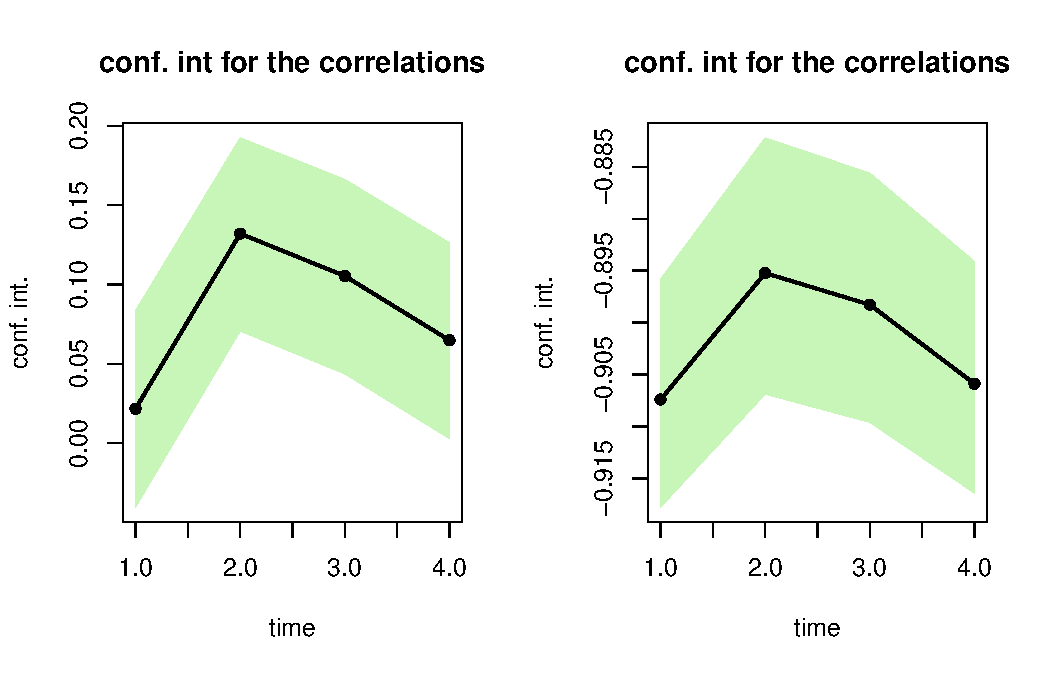
\includegraphics[width=\maxwidth]{figure/example_simshocks_3-1} 

}



\end{knitrout}

Now with other types of dependences, namely rotated versions of the Clayton copula :

\begin{knitrout}
\definecolor{shadecolor}{rgb}{0.969, 0.969, 0.969}\color{fgcolor}\begin{kframe}
\begin{alltt}
\hlcom{# Family : Rotated Clayton (180 degrees)}
\hlstd{fam2} \hlkwb{<-} \hlnum{13}
\hlstd{par0_3} \hlkwb{<-} \hlnum{2}

\hlcom{# Family : Rotated Clayton (90 degrees)}
\hlstd{fam3} \hlkwb{<-} \hlnum{23}
\hlstd{par0_4} \hlkwb{<-} \hlopt{-}\hlnum{2}

\hlcom{# number of simulations}
\hlstd{nb} \hlkwb{<-} \hlnum{200}

\hlcom{# Simulation of shocks for the d risk factors}
\hlstd{s0_par3} \hlkwb{<-} \hlkwd{simshocks}\hlstd{(}\hlkwc{n} \hlstd{= nb,} \hlkwc{horizon} \hlstd{=} \hlnum{4}\hlstd{,}
\hlkwc{family} \hlstd{= fam2,} \hlkwc{par} \hlstd{= par0_3)}

\hlstd{s0_par4} \hlkwb{<-} \hlkwd{simshocks}\hlstd{(}\hlkwc{n} \hlstd{= nb,} \hlkwc{horizon} \hlstd{=} \hlnum{4}\hlstd{,}
\hlkwc{family} \hlstd{= fam3,} \hlkwc{par} \hlstd{= par0_4)}
\end{alltt}
\end{kframe}
\end{knitrout}

There's a nice function from the package, \code{esgplotshocks}, that helps you in visualizing  dependence between shocks (inspired by \href{http://rforpublichealth.blogspot.fr/2014/02/ggplot2-cheatsheet-for-visualizing.html}{this blog post}) : 

\begin{knitrout}
\definecolor{shadecolor}{rgb}{0.969, 0.969, 0.969}\color{fgcolor}\begin{kframe}
\begin{alltt}
\hlkwd{esgplotshocks}\hlstd{(s0_par3, s0_par4)}
\end{alltt}
\end{kframe}

{\centering 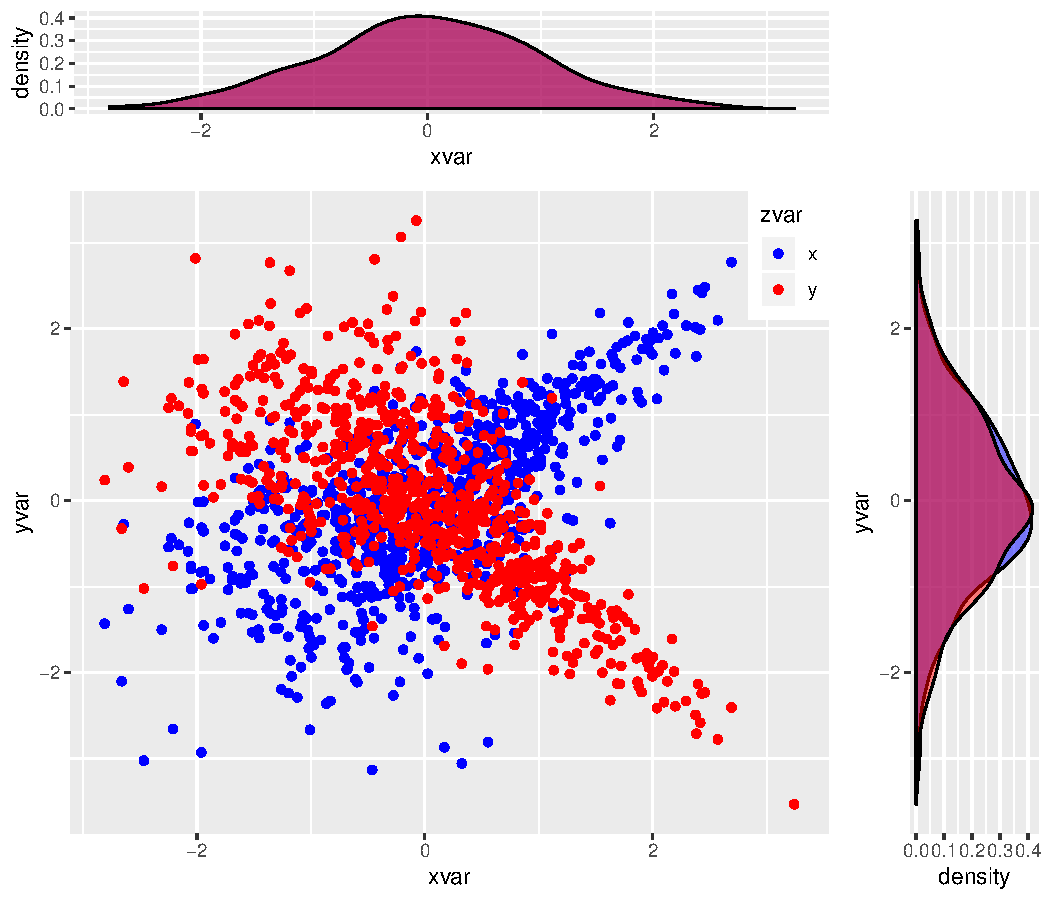
\includegraphics[width=\maxwidth]{figure/example_simshocks_5-1} 

}



\end{knitrout}

\newpage

\subsection{Example with \code{simdiff} and \code{simshocks} : Option pricing under the  Bates model (SVJD) for equity}
\label{sec:examplesimulation}

SVJD stands for Stochastic Volatility with Jump Diffusion. In this model, the volatility of the asset's price evolves as a CIR process. The price itself is a Geometric Brownian motion between jumps, arising from a Poisson process. Here, we consider jumps with lognormal magnitude.  

\medskip

{\bf The model}

\begin{eqnarray*}
dS(t) &=& (r - \lambda \mu_Z) S(t) dt + \sqrt{v(t)} S(t) dW(t)^{(1)} + (J - 1) dN(t)\\
dv(t) &=& \kappa(\theta - v(t)) dt + \sigma \sqrt{v(t)} dW(t)^{(2)}\\
dW(t)^{(1)} dW(t)^{(2)} &=& \rho dt
\end{eqnarray*}

We use the package \code{fOptions} to compute options' prices from market implied volatility : 
\begin{knitrout}
\definecolor{shadecolor}{rgb}{0.969, 0.969, 0.969}\color{fgcolor}\begin{kframe}
\begin{alltt}
\hlkwd{library}\hlstd{(fOptions)}
\end{alltt}
\end{kframe}
\end{knitrout}

The parameters of Bates model are : 
\begin{knitrout}
\definecolor{shadecolor}{rgb}{0.969, 0.969, 0.969}\color{fgcolor}\begin{kframe}
\begin{alltt}
\hlcom{# Spot variance}
\hlstd{V0} \hlkwb{<-} \hlnum{0.1372}
\hlcom{# mean-reversion speed}
\hlstd{kappa} \hlkwb{<-} \hlnum{9.5110}\hlopt{/}\hlnum{100}
\hlcom{# long-term variance}
\hlstd{theta} \hlkwb{<-} \hlnum{0.0285}
\hlcom{# volatility of volatility}
\hlstd{volvol} \hlkwb{<-} \hlnum{0.8010}\hlopt{/}\hlnum{100}
\hlcom{# Correlation between stoch. vol and prices}
\hlstd{rho} \hlkwb{<-} \hlopt{-}\hlnum{0.5483}
\hlcom{# Intensity of the Poisson process}
\hlstd{lambda} \hlkwb{<-} \hlnum{0.3635}
\hlcom{# mean and vol of the merton jumps diffusion}
\hlstd{mu_J} \hlkwb{<-} \hlopt{-}\hlnum{0.2459}
\hlstd{sigma_J} \hlkwb{<-} \hlnum{0.2547}\hlopt{/}\hlnum{100}
\hlstd{m} \hlkwb{<-} \hlkwd{exp}\hlstd{(mu_J} \hlopt{+} \hlnum{0.5}\hlopt{*}\hlstd{(sigma_J}\hlopt{^}\hlnum{2}\hlstd{))} \hlopt{-} \hlnum{1}
\hlcom{# Initial stock price}
\hlstd{S0} \hlkwb{<-} \hlnum{4468.17}
\hlcom{# Initial short rate}
\hlstd{r0} \hlkwb{<-} \hlnum{0.0357}
\end{alltt}
\end{kframe}
\end{knitrout}

Now we make \code{300} simulations of shocks and diffusions, on a weekly basis, from today, up to year 1. The shocks are simulated by using a variance reduction technique : antithetic variates (argument \code{method}). 

\begin{knitrout}
\definecolor{shadecolor}{rgb}{0.969, 0.969, 0.969}\color{fgcolor}\begin{kframe}
\begin{alltt}
\hlstd{n} \hlkwb{<-} \hlnum{300}
\hlstd{horizon} \hlkwb{<-} \hlnum{1}
\hlstd{freq} \hlkwb{<-} \hlstr{"weekly"}

\hlcom{# Simulation of shocks, with antithetic variates}
\hlstd{shocks} \hlkwb{<-} \hlkwd{simshocks}\hlstd{(}\hlkwc{n} \hlstd{= n,} \hlkwc{horizon} \hlstd{= horizon,}
          \hlkwc{frequency} \hlstd{= freq,}
          \hlkwc{method} \hlstd{=} \hlstr{"anti"}\hlstd{,}
          \hlkwc{family} \hlstd{=} \hlnum{1}\hlstd{,} \hlkwc{par} \hlstd{= rho)}

\hlcom{# Vol simulation}
\hlstd{sim_vol} \hlkwb{<-} \hlkwd{simdiff}\hlstd{(}\hlkwc{n} \hlstd{= n,} \hlkwc{horizon} \hlstd{= horizon,}
                   \hlkwc{frequency} \hlstd{= freq,} \hlkwc{model} \hlstd{=} \hlstr{"CIR"}\hlstd{,} \hlkwc{x0} \hlstd{= V0,}
                   \hlkwc{theta1} \hlstd{= kappa}\hlopt{*}\hlstd{theta,} \hlkwc{theta2} \hlstd{= kappa,}
                   \hlkwc{theta3} \hlstd{= volvol,}
                    \hlkwc{eps} \hlstd{= shocks[[}\hlnum{1}\hlstd{]])}

\hlcom{# Plotting the volatility (only for a low number of simulations)}
\hlkwd{esgplotts}\hlstd{(sim_vol)}
\end{alltt}
\end{kframe}
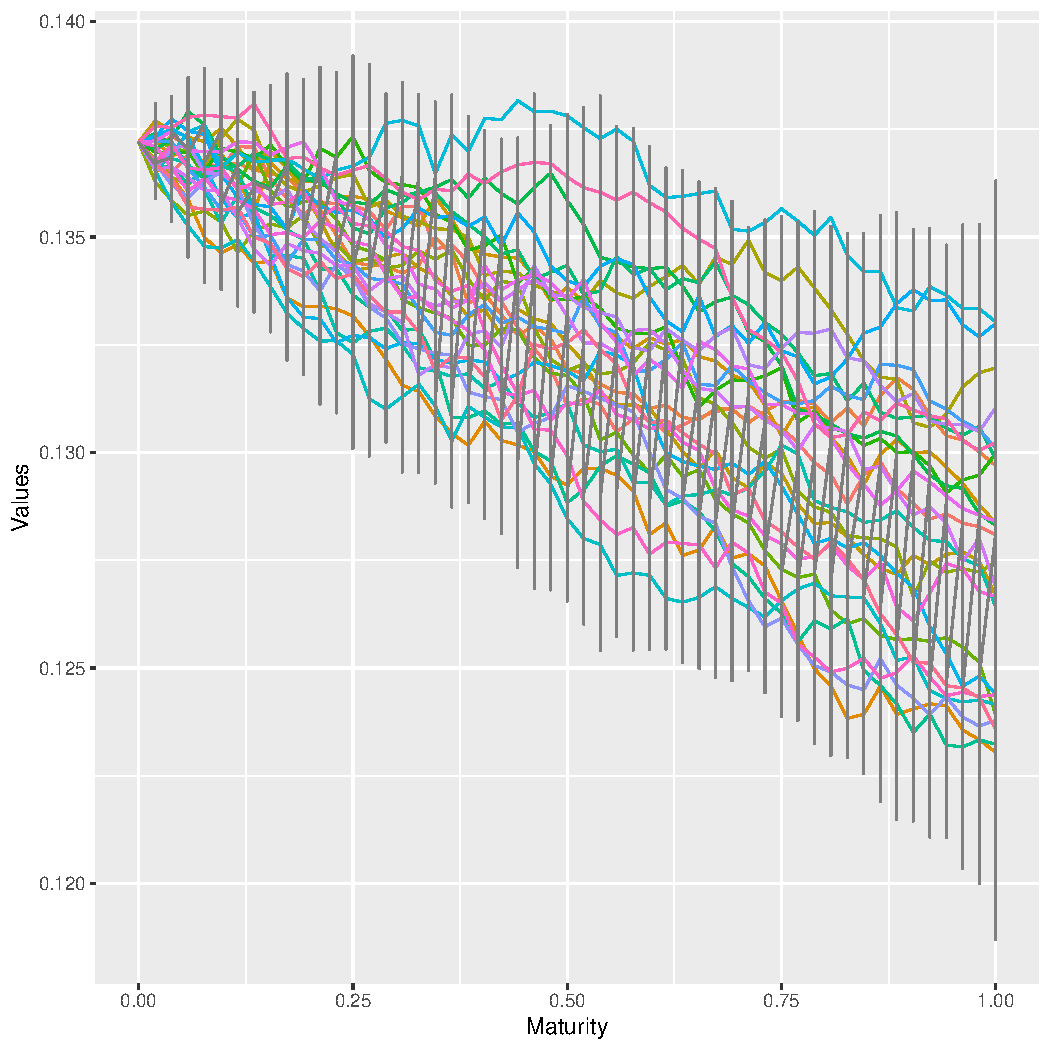
\includegraphics[width=\maxwidth]{figure/_example_SVJD_2-1} 

\end{knitrout}

Finally, the price's simulation takes {\bf exactly the same parameters} \code{n, horizon, frequency} as \code{simshocks} and \code{simdiff}, and the volatility is embedded through \code{theta2}.

\begin{knitrout}
\definecolor{shadecolor}{rgb}{0.969, 0.969, 0.969}\color{fgcolor}\begin{kframe}
\begin{alltt}
\hlcom{# prices simulation}
\hlstd{sim_price} \hlkwb{<-} \hlkwd{simdiff}\hlstd{(}\hlkwc{n} \hlstd{= n,} \hlkwc{horizon} \hlstd{= horizon,}
                     \hlkwc{frequency} \hlstd{= freq,} \hlkwc{model} \hlstd{=} \hlstr{"GBM"}\hlstd{,} \hlkwc{x0} \hlstd{= S0,}
                     \hlkwc{theta1} \hlstd{= r0} \hlopt{-} \hlstd{lambda}\hlopt{*}\hlstd{m,} \hlkwc{theta2} \hlstd{= sim_vol,}
                     \hlkwc{lambda} \hlstd{= lambda,} \hlkwc{mu_z} \hlstd{= mu_J,}
                     \hlkwc{sigma_z} \hlstd{= sigma_J,}
                     \hlkwc{eps} \hlstd{= shocks[[}\hlnum{2}\hlstd{]])}
\end{alltt}


{\ttfamily\noindent\bfseries\color{errorcolor}{\#\# Error in simdiff(n = n, horizon = horizon, frequency = freq, model = "{}GBM"{}, : unused arguments (mu\_z = mu\_J, sigma\_z = sigma\_J)}}\end{kframe}
\end{knitrout}

We can clearly see the prices jumping with \code{matplot}. But \code{esgplotbands}, offering a view of the paths by percentiles, will be more useful for thousands of simulations : 

\begin{knitrout}
\definecolor{shadecolor}{rgb}{0.969, 0.969, 0.969}\color{fgcolor}\begin{kframe}
\begin{alltt}
\hlkwd{par}\hlstd{(}\hlkwc{mfrow}\hlstd{=}\hlkwd{c}\hlstd{(}\hlnum{2}\hlstd{,} \hlnum{1}\hlstd{))}
\hlkwd{matplot}\hlstd{(}\hlkwd{time}\hlstd{(sim_price), sim_price,} \hlkwc{type} \hlstd{=} \hlstr{'l'}\hlstd{,}
        \hlkwc{main} \hlstd{=} \hlstr{"with matplot"}\hlstd{)}
\end{alltt}


{\ttfamily\noindent\bfseries\color{errorcolor}{\#\# Error in time(sim\_price): object 'sim\_price' not found}}\begin{alltt}
\hlkwd{esgplotbands}\hlstd{(sim_price,} \hlkwc{main} \hlstd{=} \hlstr{"with esgplotbands"}\hlstd{,} \hlkwc{xlab} \hlstd{=} \hlstr{"time"}\hlstd{,}
             \hlkwc{ylab} \hlstd{=} \hlstr{"values"}\hlstd{)}
\end{alltt}


{\ttfamily\noindent\bfseries\color{errorcolor}{\#\# Error in is.ts(x): object 'sim\_price' not found}}\end{kframe}
\end{knitrout}

Now, we would like to verify the convergence of the estimated discounted prices to the initial asset price : 

\begin{equation}
\frac{1}{N}\sum_{i = 1}^N e^{-rT} S_T^{(i)} \longrightarrow \EE[e^{-rT}S_T] = S_0
\end{equation}

where $N$ is the number of simulations, $r$ is the constant risk free rate, and $T$ is a maturity of 2 weeks. 

\begin{knitrout}
\definecolor{shadecolor}{rgb}{0.969, 0.969, 0.969}\color{fgcolor}\begin{kframe}
\begin{alltt}
\hlcom{# Discounted Monte Carlo price}
\hlkwd{as.numeric}\hlstd{(}\hlkwd{esgmcprices}\hlstd{(r0, sim_price,} \hlnum{2}\hlopt{/}\hlnum{52}\hlstd{))}
\end{alltt}


{\ttfamily\noindent\bfseries\color{errorcolor}{\#\# Error in is.ts(X): object 'sim\_price' not found}}\begin{alltt}
\hlcom{# Inital price}
\hlstd{S0}
\end{alltt}
\begin{verbatim}
## [1] 4468.17
\end{verbatim}
\begin{alltt}
\hlcom{# pct. difference}
\hlkwd{as.numeric}\hlstd{((}\hlkwd{esgmcprices}\hlstd{(r0, sim_price,} \hlnum{2}\hlopt{/}\hlnum{52}\hlstd{)}\hlopt{/}\hlstd{S0} \hlopt{-} \hlnum{1}\hlstd{)}\hlopt{*}\hlnum{100}\hlstd{)}
\end{alltt}


{\ttfamily\noindent\bfseries\color{errorcolor}{\#\# Error in is.ts(X): object 'sim\_price' not found}}\end{kframe}
\end{knitrout}

One would also want to see how fast is the convergence towards $S0$ :
\begin{knitrout}
\definecolor{shadecolor}{rgb}{0.969, 0.969, 0.969}\color{fgcolor}\begin{kframe}
\begin{alltt}
\hlcom{# convergence of the discounted price}
\hlkwd{esgmccv}\hlstd{(r0, sim_price,} \hlnum{2}\hlopt{/}\hlnum{52}\hlstd{,}
        \hlkwc{main} \hlstd{=} \hlstr{"Convergence towards the initial \textbackslash{}n asset price"}\hlstd{)}
\end{alltt}


{\ttfamily\noindent\bfseries\color{errorcolor}{\#\# Error in is.ts(X): object 'sim\_price' not found}}\end{kframe}
\end{knitrout}

\code{esgmcprices} and \code{esgmccv} give information about the mean, but a statistical test gives more information.  

\begin{knitrout}
\definecolor{shadecolor}{rgb}{0.969, 0.969, 0.969}\color{fgcolor}\begin{kframe}
\begin{alltt}
\hlstd{martingaletest_sim_price} \hlkwb{<-} \hlkwd{esgmartingaletest}\hlstd{(}\hlkwc{r} \hlstd{= r0,}
                                              \hlkwc{X} \hlstd{= sim_price,}
                                              \hlkwc{p0} \hlstd{= S0)}
\end{alltt}


{\ttfamily\noindent\bfseries\color{errorcolor}{\#\# Error in deltat(X): object 'sim\_price' not found}}\end{kframe}
\end{knitrout}

\code{esgmartingaletest} computes for each $T$, a Student's t-test of 
$$H_0 : \EE[e^{-rT}S_T - S_0] = 0$$
versus the alternative hypothesis that the mean is not $0$, at a given confidence level (default is $95\%$).

\medskip

\code{esgmartingaletest} also provides p-values, and confidence intervals for the mean value. If all the confidence intervals contain $0$, then the null hypothesis is not rejected at the given level, let's say $95\%$. Which means that there are less than $5$ chances out of $100$ to be wrong by saying that the true mean of the distribution is $0$. 

\medskip
\code{esgplotbands} gives a visualization of the confidence intervals, as well as the average discounted prices. 

\begin{knitrout}
\definecolor{shadecolor}{rgb}{0.969, 0.969, 0.969}\color{fgcolor}\begin{kframe}
\begin{alltt}
\hlkwd{esgplotbands}\hlstd{(martingaletest_sim_price)}
\end{alltt}


{\ttfamily\noindent\bfseries\color{errorcolor}{\#\# Error in is.ts(x): object 'martingaletest\_sim\_price' not found}}\end{kframe}
\end{knitrout}

Now, we price a call option under the Bates model :

\begin{knitrout}
\definecolor{shadecolor}{rgb}{0.969, 0.969, 0.969}\color{fgcolor}\begin{kframe}
\begin{alltt}
\hlcom{# Option pricing}

\hlcom{# Strike}
\hlstd{K} \hlkwb{<-} \hlnum{3400}
\hlstd{Kts} \hlkwb{<-} \hlkwd{ts}\hlstd{(}\hlkwd{matrix}\hlstd{(K,} \hlkwd{nrow}\hlstd{(sim_price),} \hlkwd{ncol}\hlstd{(sim_price)),}
               \hlkwc{start} \hlstd{=} \hlkwd{start}\hlstd{(sim_price),}
          \hlkwc{deltat} \hlstd{=} \hlkwd{deltat}\hlstd{(sim_price),}
          \hlkwc{end} \hlstd{=} \hlkwd{end}\hlstd{(sim_price))}
\end{alltt}


{\ttfamily\noindent\bfseries\color{errorcolor}{\#\# Error in nrow(sim\_price): object 'sim\_price' not found}}\begin{alltt}
\hlcom{# Implied volatility}
\hlstd{sigma_imp} \hlkwb{<-} \hlnum{0.6625}

\hlcom{#Maturity}
\hlstd{maturity} \hlkwb{<-} \hlnum{2}\hlopt{/}\hlnum{52}

\hlcom{# payoff at maturity}
\hlstd{payoff_} \hlkwb{<-} \hlstd{(sim_price} \hlopt{-} \hlstd{Kts)}\hlopt{*}\hlstd{(sim_price} \hlopt{>} \hlstd{Kts)}
\end{alltt}


{\ttfamily\noindent\bfseries\color{errorcolor}{\#\# Error in eval(expr, envir, enclos): object 'sim\_price' not found}}\begin{alltt}
\hlstd{payoff} \hlkwb{<-} \hlkwd{window}\hlstd{(payoff_,}
             \hlkwc{start} \hlstd{=} \hlkwd{deltat}\hlstd{(sim_price),}
             \hlkwc{deltat} \hlstd{=} \hlkwd{deltat}\hlstd{(sim_price),}
             \hlkwc{names} \hlstd{=} \hlkwd{paste0}\hlstd{(}\hlstr{"Series "}\hlstd{,} \hlnum{1}\hlopt{:}\hlstd{n))}
\end{alltt}


{\ttfamily\noindent\bfseries\color{errorcolor}{\#\# Error in window(payoff\_, start = deltat(sim\_price), deltat = deltat(sim\_price), : object 'payoff\_' not found}}\begin{alltt}
\hlcom{# True price}
\hlstd{c0} \hlkwb{<-} \hlkwd{GBSOption}\hlstd{(}\hlstr{"c"}\hlstd{,} \hlkwc{S} \hlstd{= S0,} \hlkwc{X} \hlstd{= K,} \hlkwc{Time} \hlstd{= maturity,} \hlkwc{r} \hlstd{= r0,}
                \hlkwc{b} \hlstd{=} \hlnum{0}\hlstd{,} \hlkwc{sigma} \hlstd{= sigma_imp)}
\hlkwd{print}\hlstd{(c0}\hlopt{@}\hlkwc{price}\hlstd{)}
\end{alltt}
\begin{verbatim}
## [1] 1069.945
\end{verbatim}
\begin{alltt}
\hlcom{# Monte Carlo price}
\hlkwd{as.numeric}\hlstd{(}\hlkwd{esgmcprices}\hlstd{(}\hlkwc{r} \hlstd{= r0,} \hlkwc{X} \hlstd{= payoff, maturity))}
\end{alltt}


{\ttfamily\noindent\bfseries\color{errorcolor}{\#\# Error in is.ts(X): object 'payoff' not found}}\begin{alltt}
\hlcom{# pct. difference}
\hlkwd{as.numeric}\hlstd{((}\hlkwd{esgmcprices}\hlstd{(}\hlkwc{r} \hlstd{= r0,} \hlkwc{X} \hlstd{= payoff,}
             \hlkwc{maturity} \hlstd{= maturity)}\hlopt{/}\hlstd{c0}\hlopt{@}\hlkwc{price} \hlopt{-} \hlnum{1}\hlstd{)}\hlopt{*}\hlnum{100}\hlstd{)}
\end{alltt}


{\ttfamily\noindent\bfseries\color{errorcolor}{\#\# Error in is.ts(X): object 'payoff' not found}}\begin{alltt}
\hlcom{# Convergence towards the option price}
\hlkwd{esgmccv}\hlstd{(}\hlkwc{r} \hlstd{= r0,} \hlkwc{X} \hlstd{= payoff,} \hlkwc{maturity} \hlstd{= maturity,}
        \hlkwc{main} \hlstd{=} \hlstr{"Convergence towards the call \textbackslash{}n option price"}\hlstd{)}
\end{alltt}


{\ttfamily\noindent\bfseries\color{errorcolor}{\#\# Error in is.ts(X): object 'payoff' not found}}\end{kframe}
\end{knitrout}

\newpage

\nocite{bates1996jumps}
\nocite{black1973pricing}
\nocite{brechmann2012risk}
\nocite{brechmann2013modeling}
\nocite{brigo2006interest}
\nocite{cox1985theory}
\nocite{eddelbuettel2011rcpp}
\nocite{glasserman2004monte}
\nocite{iacus2008simulation}
\nocite{kou2002jump}
\nocite{merton1976option}
\nocite{uhlenbeck1930theory}
\nocite{vasicek1977equilibrium}
\nocite{wickham2009ggplot2}
\bibliographystyle{jss}
\bibliography{mabiblio}

\end{document}
